\section{Behaviour as \texorpdfstring{$p\to\tfrac12^-$}{p to 1/2}}
\label{a:sec:asymptotic}

The bounds of \cref{a:eq:Abounds} show that $A(p)$ is of order $\varepsilon$, but
leave a factor of two unresolved. The series \cref{a:eq:Aseries} determines the
leading constant and, with a little more care, the order of the first relative
correction.

The idea is visible before any estimates are made. Fix $\varepsilon$ small. The
summand $r^n/(2-S_n)$ involves two decays on very different scales. The geometric
factor $r^n = (1-\varepsilon)^n$ decays on the scale $n\sim1/\varepsilon$, which
is large. The survival probability $S_n$, by contrast, is close to its critical
behaviour $S_n\sim2/n$ over that whole range, and so has already fallen to near
zero after $O(1)$ generations. For the overwhelming majority of the terms that
carry weight, therefore, $S_n\approx0$ and the summand is approximately $r^n/2$.
Summing,
\begin{equation*}
\sum_{n=0}^{\infty}\frac{r^n}{2-S_n}
\;\approx\;
\frac12\sum_{n=0}^{\infty}r^n = \frac{1}{2\varepsilon},
\end{equation*}
so $1/A(p)\sim1/(2\varepsilon)$ and
\begin{equation}
\label{a:eq:Aasym}
\boxed{\;A(p)\sim2\varepsilon = 2(1-2p)\qquad\text{as }p\to\tfrac12^-.\;}
\end{equation}
Equivalently $1/A(p)\sim1/\bigl(2(1-2p)\bigr)$: the quasi-stationary mean diverges
like the reciprocal of the distance from criticality. In particular $A(p)$ meets
the axis at $p=\tfrac12$ with gradient $-4$, a fact used repeatedly below as a
test of candidate formulae. The heuristic is now made rigorous, with the order of
the remainder.

\begin{theorem}[Near-critical asymptotic]
\label{a:thm:nearcrit}
As $p\uparrow\tfrac12$, with $\varepsilon=1-2p\downarrow0$,
\begin{equation}
\label{a:eq:Anearcrit}
A(p) = 2\varepsilon\Bigl[1+O\Bigl(\varepsilon\ln\frac1\varepsilon\Bigr)\Bigr] .
\end{equation}
In particular \cref{a:eq:Aasym} holds, and
$1/A(p)\sim1/\bigl(2(1-2p)\bigr)$.
\end{theorem}

\begin{proof}
Write $r=1-\varepsilon$. The identity
\begin{equation*}
\frac{1}{2-S_n} = \frac12 + \frac{S_n}{2(2-S_n)}
\end{equation*}
turns \cref{a:eq:Aseries} into
\begin{equation}
\label{a:eq:Aseriesdecomp}
\frac1{A(p)} = 1 + \frac{1}{2\varepsilon} + D_\varepsilon,
\qquad
D_\varepsilon := \sum_{n=0}^{\infty}r^n\,\frac{S_n}{2(2-S_n)} .
\end{equation}
Only a logarithmic bound on the remainder is needed. The map
$s\mapsto ps(2-s)$ is increasing in both $p$ and $s$ on the relevant range, so
the subcritical survival probability is bounded above by its critical
counterpart, $S_n(p)\le S_n(\tfrac12)$. At $p=\tfrac12$ the recursion gives
\begin{equation*}
\frac{1}{S_{n+1}(\tfrac12)}-\frac{1}{S_n(\tfrac12)}
= \frac{1}{2(1-S_n(\tfrac12)/2)} \ge \frac12 ,
\end{equation*}
and summing the increments yields $S_n(\tfrac12)\le2/(n+2)$. Since $2-S_n\ge1$,
\begin{align}
0\le D_\varepsilon
&\le \frac12\sum_{n=0}^{\infty}r^nS_n(p)
\le \sum_{n=0}^{\infty}\frac{r^n}{n+2} \notag\\
&= \frac{-\ln(1-r)-r}{r^2}
= O\Bigl(\ln\frac1\varepsilon\Bigr) .
\label{a:eq:Depsbound}
\end{align}
Factoring $1/(2\varepsilon)$ from \cref{a:eq:Aseriesdecomp} gives
\begin{equation*}
\frac1{A(p)} = \frac{1}{2\varepsilon}\Bigl[1+2\varepsilon\{1+D_\varepsilon\}\Bigr],
\end{equation*}
in which the quantity after the leading one is
$O(\varepsilon\ln(1/\varepsilon))$; inverting proves \cref{a:eq:Anearcrit}.
\end{proof}

The proof locates the logarithm that slows convergence to the leading asymptotic.
The same result can also be reached through the continuum Riccati equation for the
survival recursion, and it is worth seeing why that route is the worse one. The
exact difference is
\begin{equation*}
S_{n+1}-S_n = (2p-1)S_n - pS_n^2
= -\varepsilon S_n - \tfrac12S_n^2 + \tfrac{\varepsilon}{2}S_n^2 ,
\end{equation*}
and dropping the $O(\varepsilon S_n^2)$ term gives
$\dd S/\dd n = -\varepsilon S-\tfrac12S^2$. Setting $u=1/S$ linearises this to
$u' = \varepsilon u+\tfrac12$, with solution
\begin{equation*}
u(n) = C\ee^{\varepsilon n} - \frac{1}{2\varepsilon},
\qquad
S(n) = \frac{1}{C\ee^{\varepsilon n}-\frac{1}{2\varepsilon}} .
\end{equation*}
Matching $S_n\sim A\ee^{-\varepsilon n}$ for small $\varepsilon$ identifies
$A=1/C$, and matching to the critical decay $S_n\sim2/n$ in the appropriate double
limit fixes $C\sim1/(2\varepsilon)$, recovering \cref{a:eq:Aasym}. Both steps are
heuristic, and the second is delicate; the series argument is preferable because it
needs no second matching at all.

\begin{remark}[Rate of approach]
\label{a:rem:rate}
Numerically, $A(p)/2\varepsilon$ approaches $1$ rather slowly. Evaluating
\cref{a:eq:prodFormula} in high precision gives $A/2\varepsilon = 0.90987$,
$0.98612$, $0.99814$, $0.99977$ and $0.999972$ at $\varepsilon=2\times10^{-2}$
down to $2\times10^{-6}$. Fitting the deficit gives
\begin{equation*}
1-\frac{A}{2\varepsilon}
\approx \varepsilon\Bigl(\ln\frac1\varepsilon+c\Bigr)
\end{equation*}
with $c\approx0.78$, though the constant is empirical and is not used in what
follows; the proved statement is the order estimate of \cref{a:thm:nearcrit}. The
logarithmic correction is why \cref{a:eq:Aasym} is a good practical surrogate only
very close to criticality, and it is what fixes the crossover point chosen in
\cref{a:sec:practical}. \Cref{a:fig:nearcrit} shows the correction over five
decades of $\varepsilon$.
\end{remark}

\begin{figure}[ht]
\centering
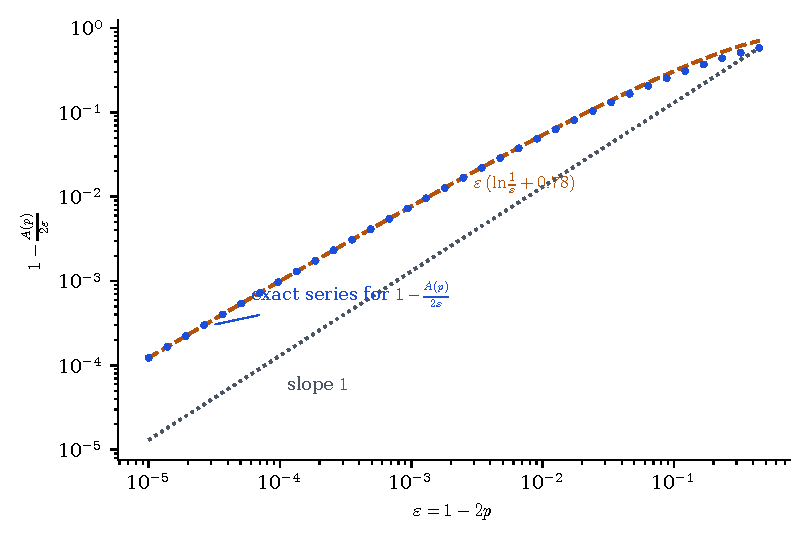
\includegraphics[width=0.86\textwidth]{figures/Ap_nearcrit.pdf}
\caption{The relative deficit $1-A(p)/2\varepsilon$ of the near-critical
asymptotic, computed from the exact series of \cref{a:prop:series} (points),
against $\varepsilon=1-2p$ on logarithmic axes. The dotted line has slope $1$;
the departure of the points from it is the logarithmic correction of
\cref{a:rem:rate}, tracked by the dashed empirical fit
$\varepsilon(\ln\frac1\varepsilon+0.78)$. The deficit is of order
$\varepsilon\ln(1/\varepsilon)$, exactly the remainder of
\cref{a:thm:nearcrit}, which is why the leading asymptotic alone is accurate
only within a few parts in $10^3$ of criticality.}
\label{a:fig:nearcrit}
\end{figure}
